\documentclass[a4paper]{article}
\usepackage[utf8]{inputenc}
\usepackage[T1]{fontenc}
\usepackage[brazil]{babel}
\usepackage{float}
\usepackage{graphicx}

\title{Etapa 5}
\author{Amilcar \and Marcelo Garlet Millani}
\date{}

\begin{document}

 \maketitle 
 
 \begin{figure}[H]
  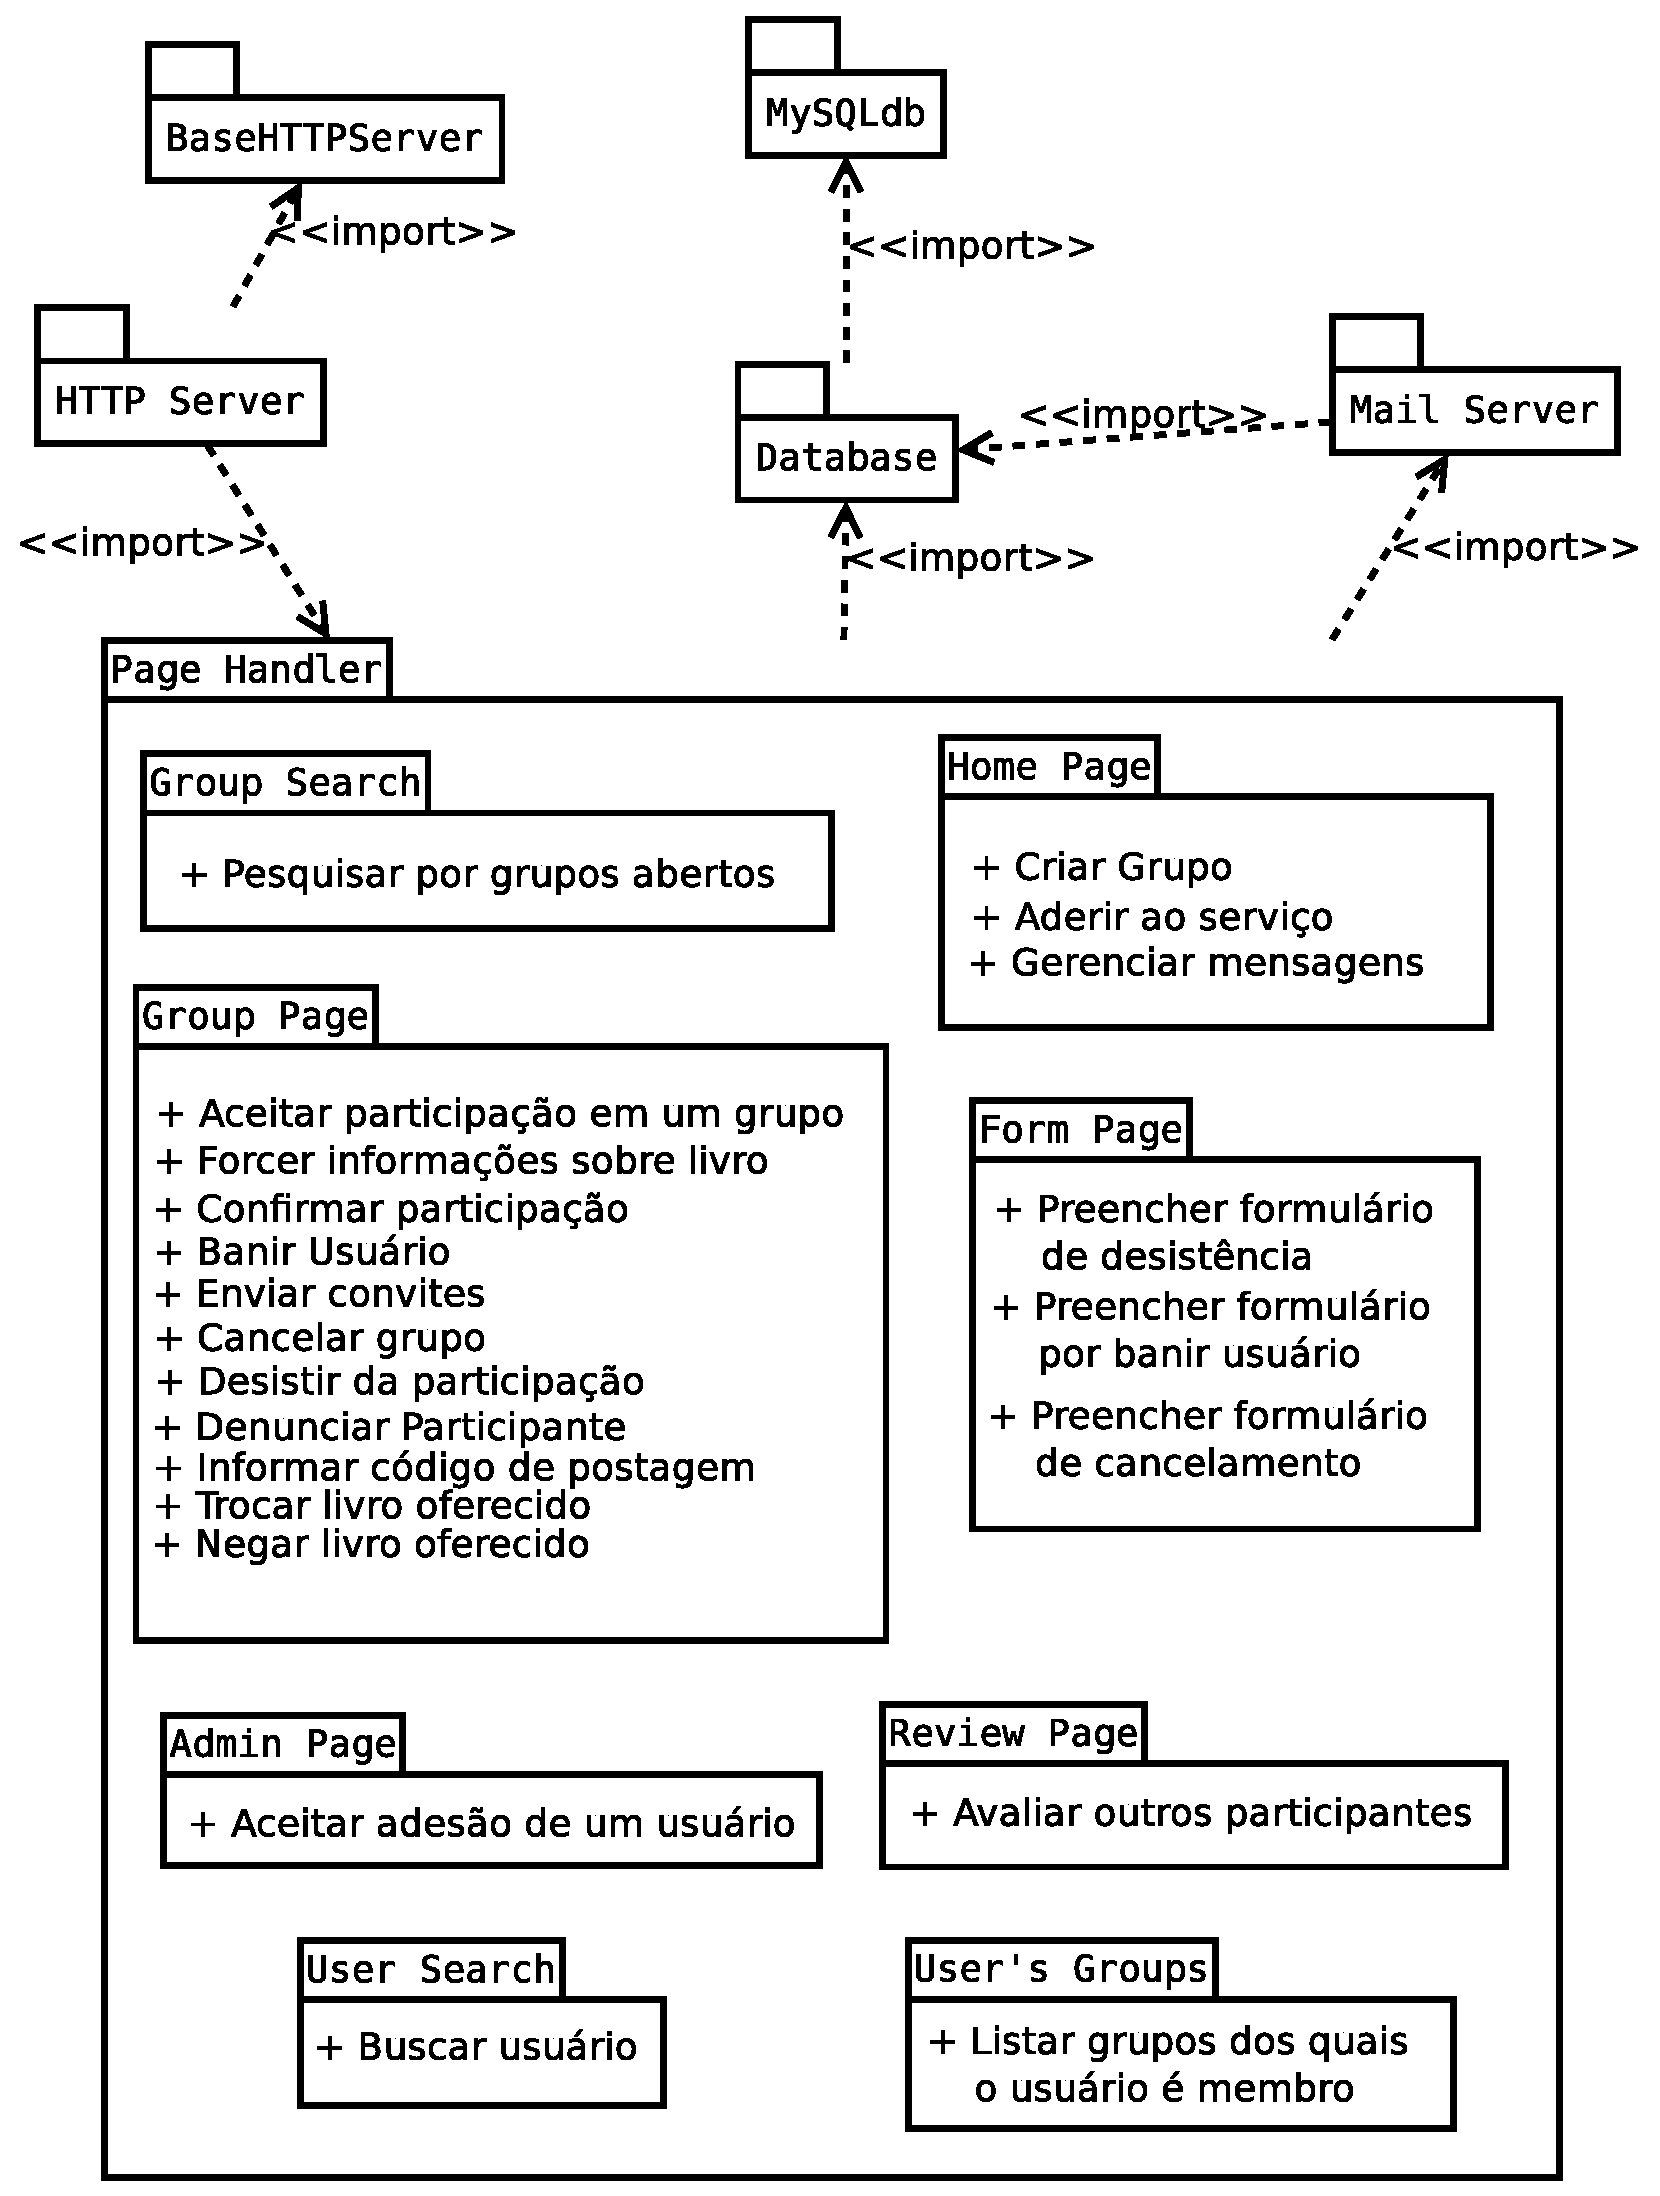
\includegraphics[totalheight=\textheight]{pacotes.eps}
  \caption{Diagrama de Pacotes},
 \end{figure}
 
 \begin{figure}[H]
  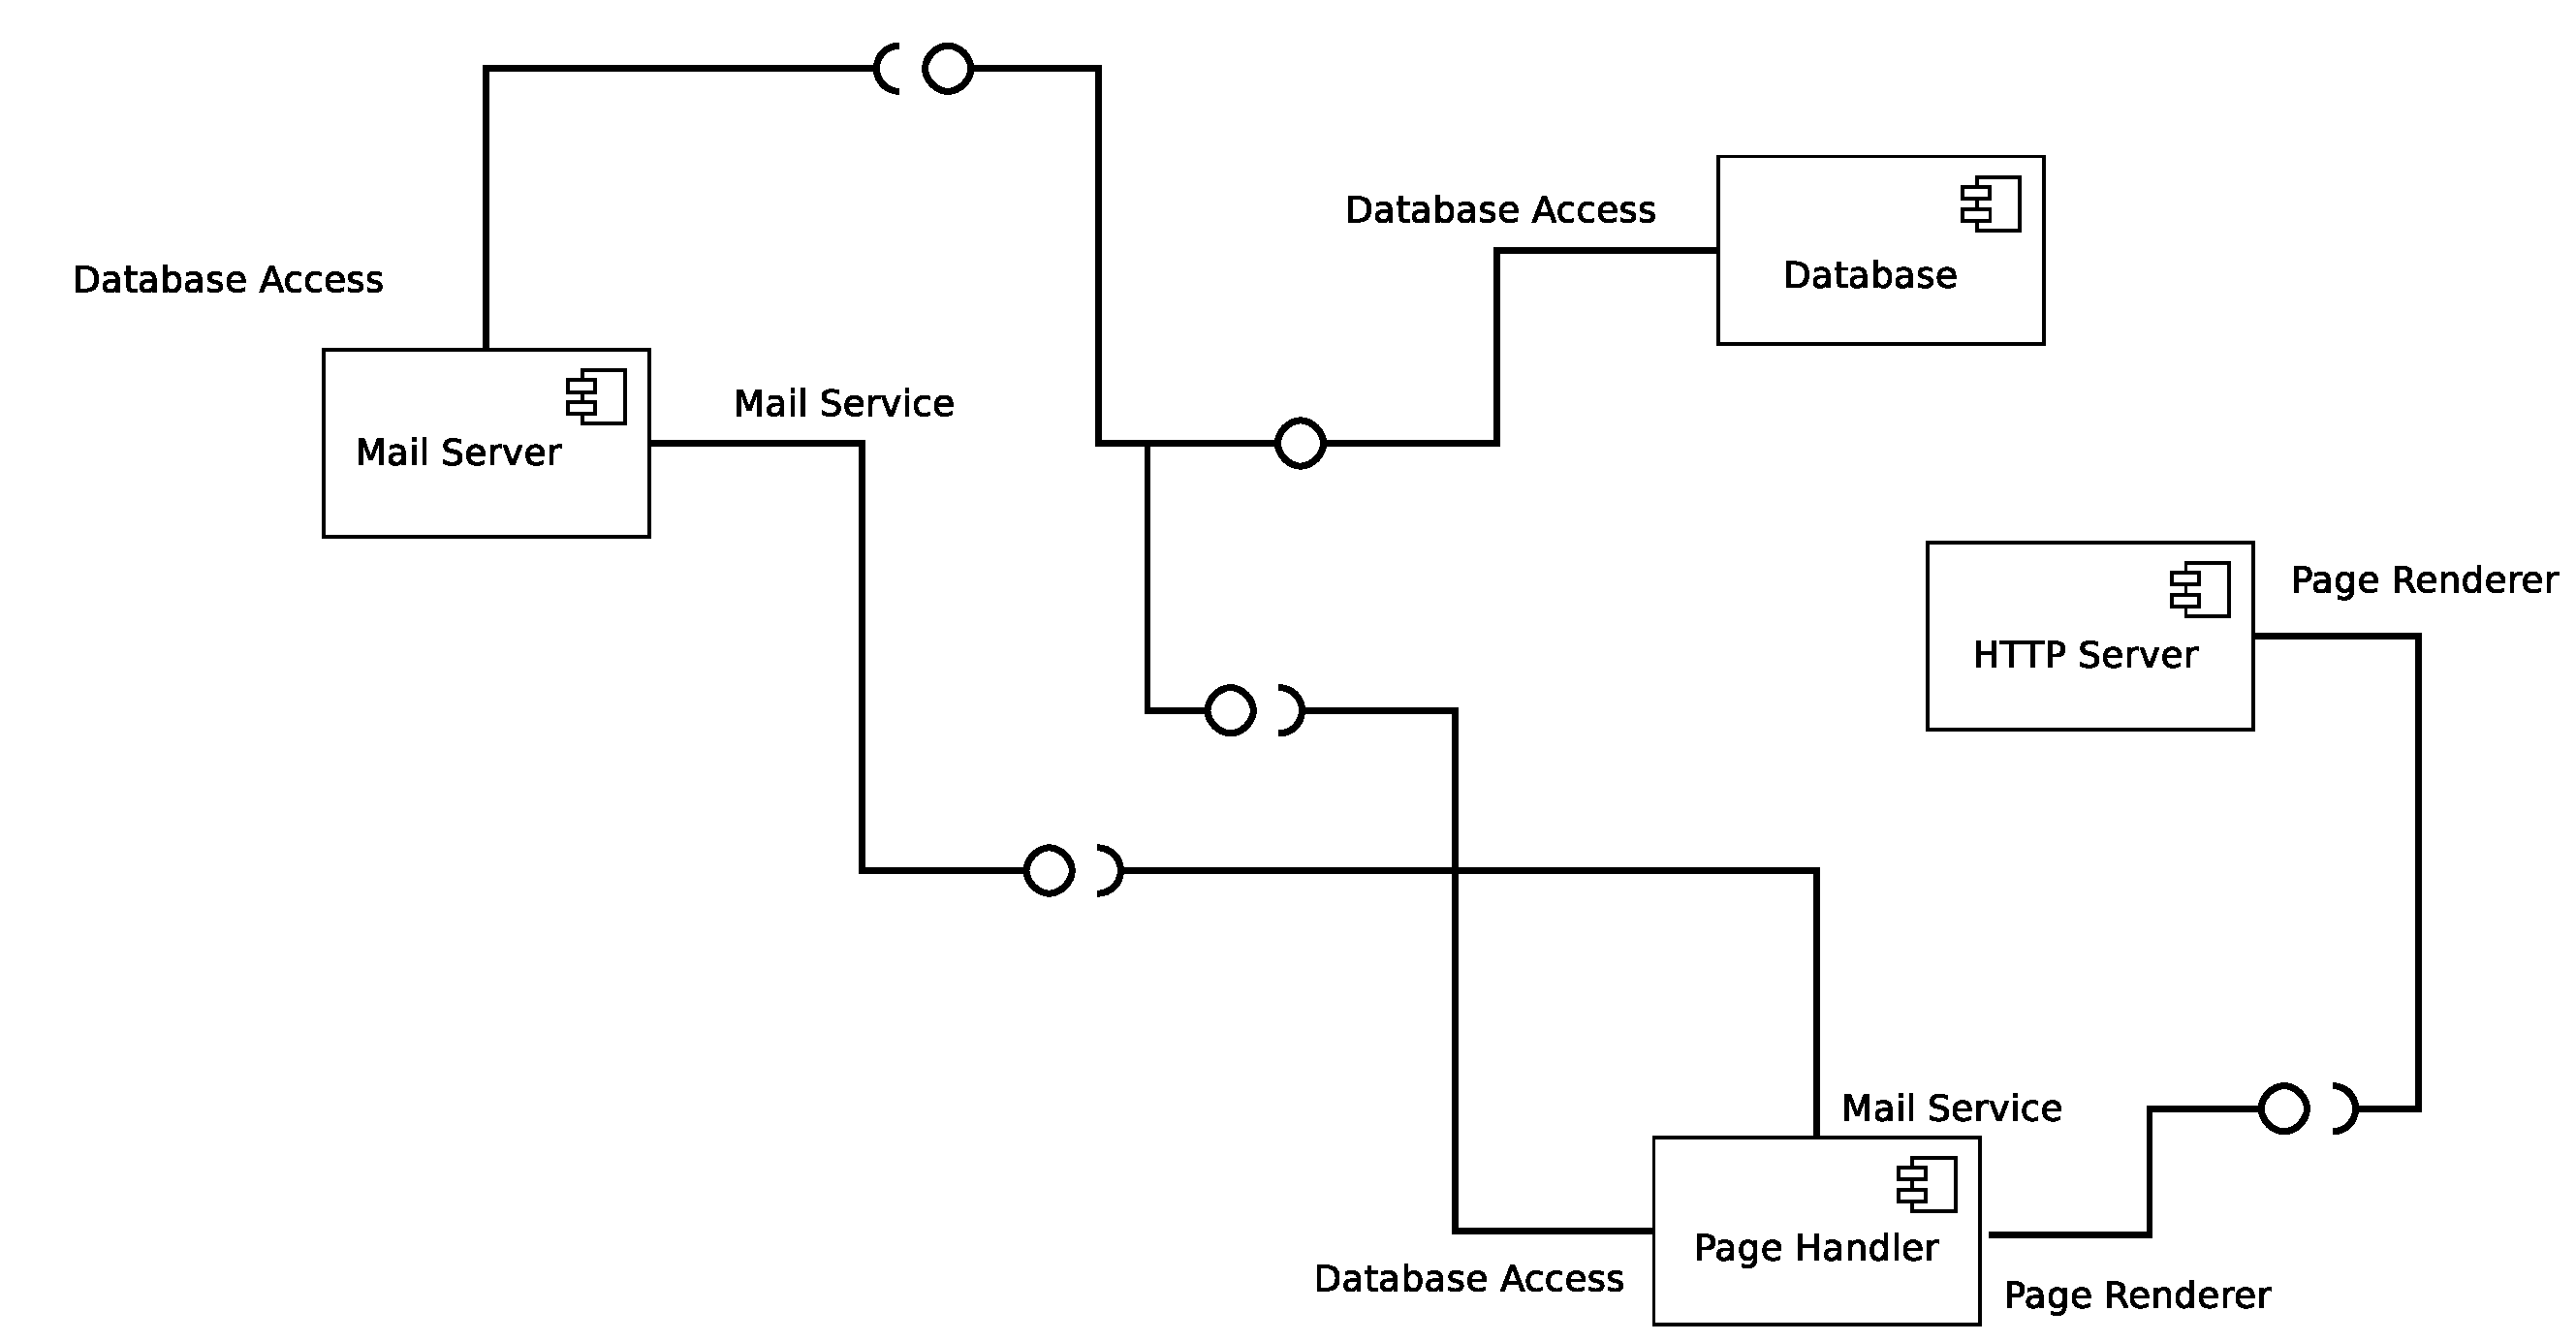
\includegraphics[angle=90,totalheight=\textheight]{componentes.eps}
  \caption{Diagrama de Componentes}
 \end{figure}
 
 \begin{figure}[H]
  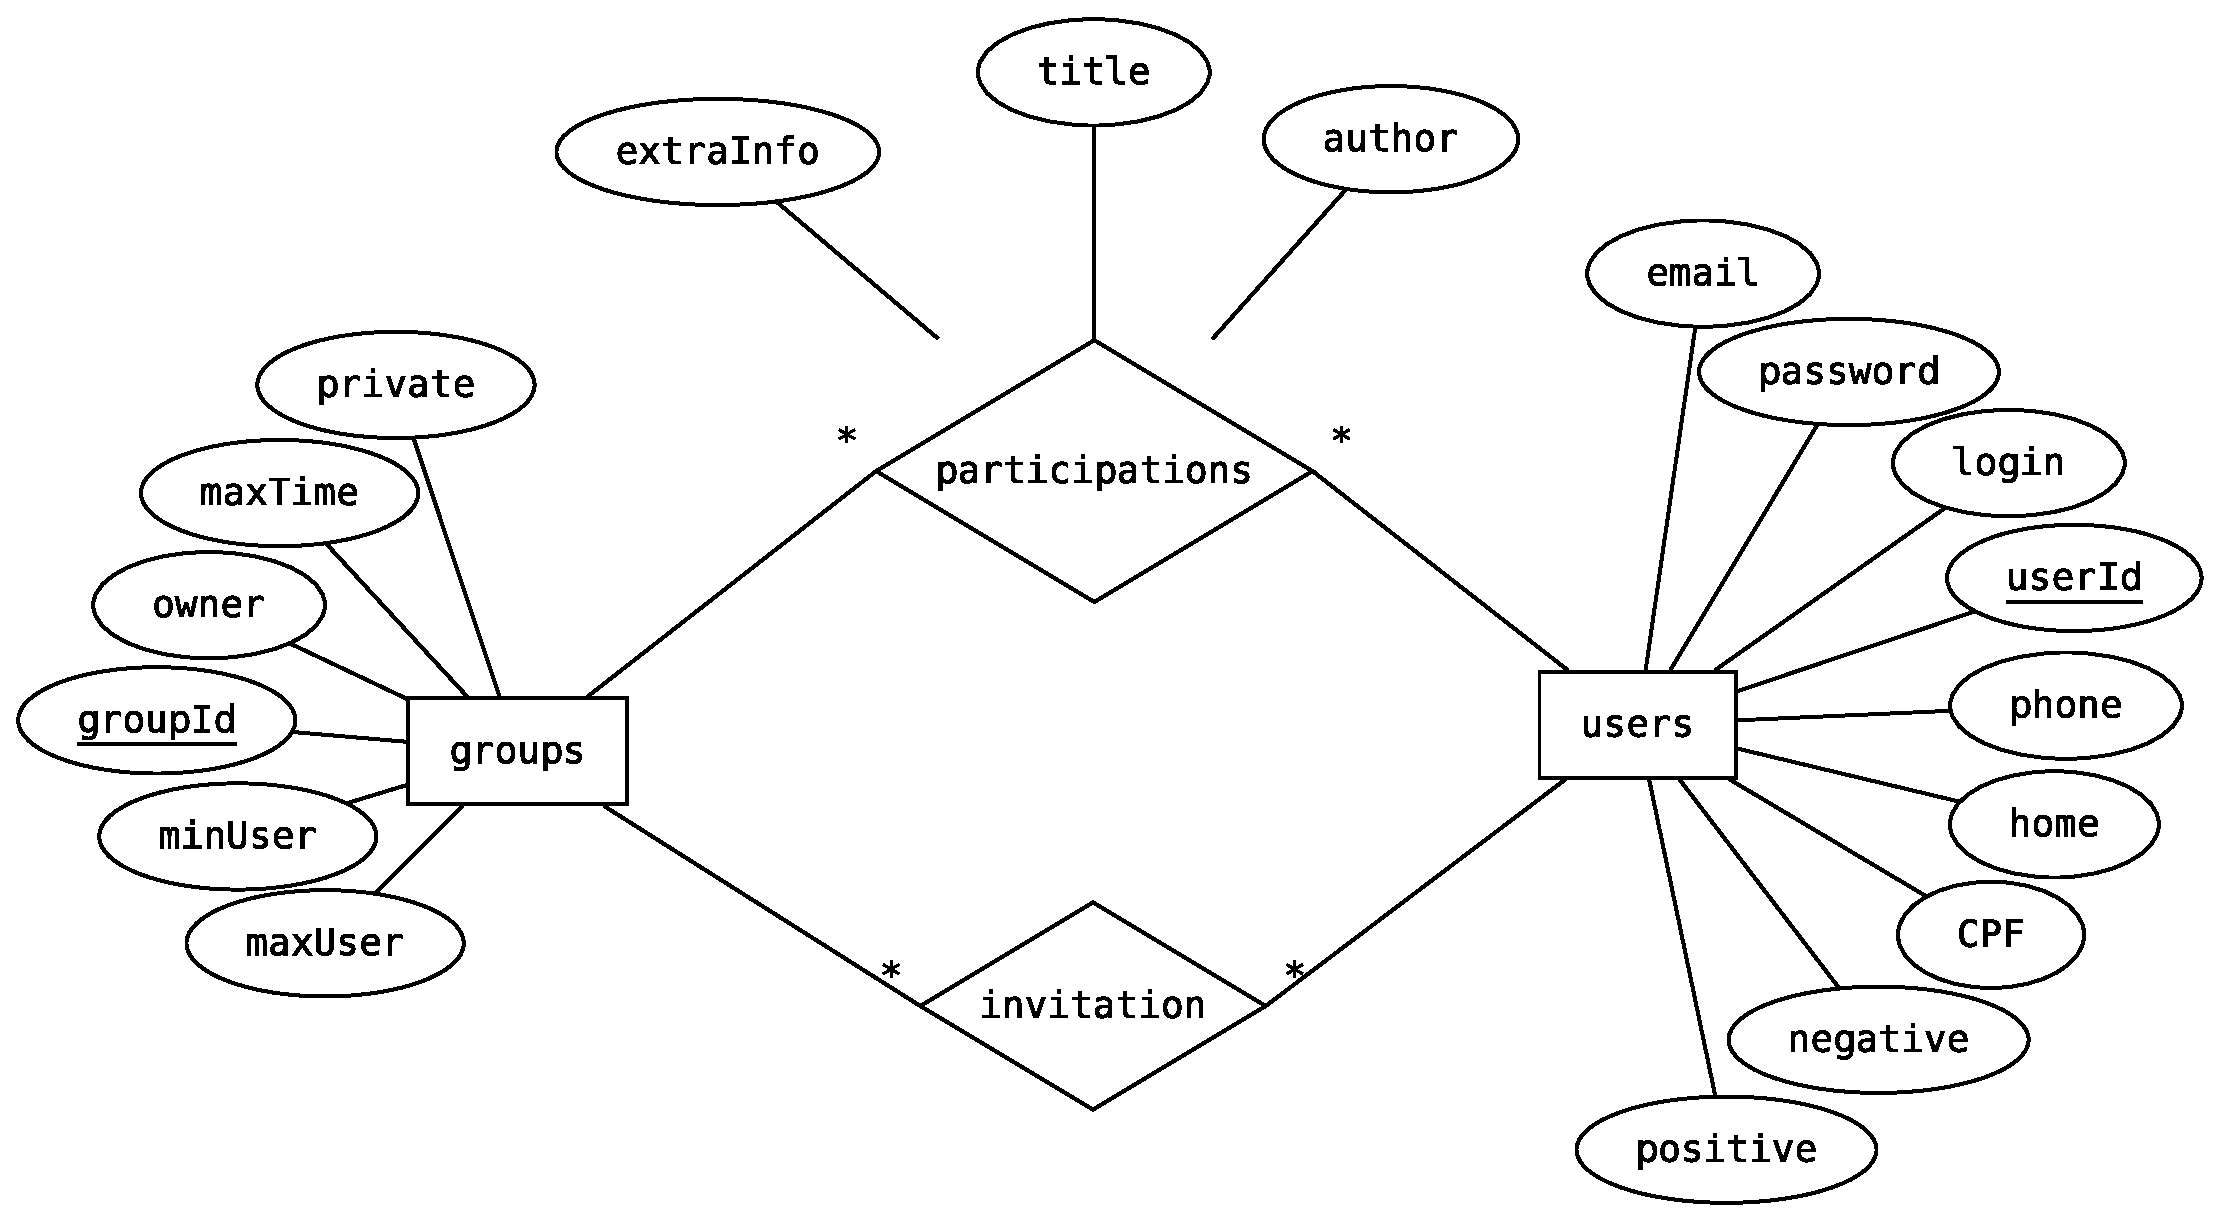
\includegraphics[angle=90,totalheight=\textheight]{modeloER.eps}
  \caption{Modelo Entidade-Relacionamento}
 \end{figure}
 
 \begin{figure}[H]
  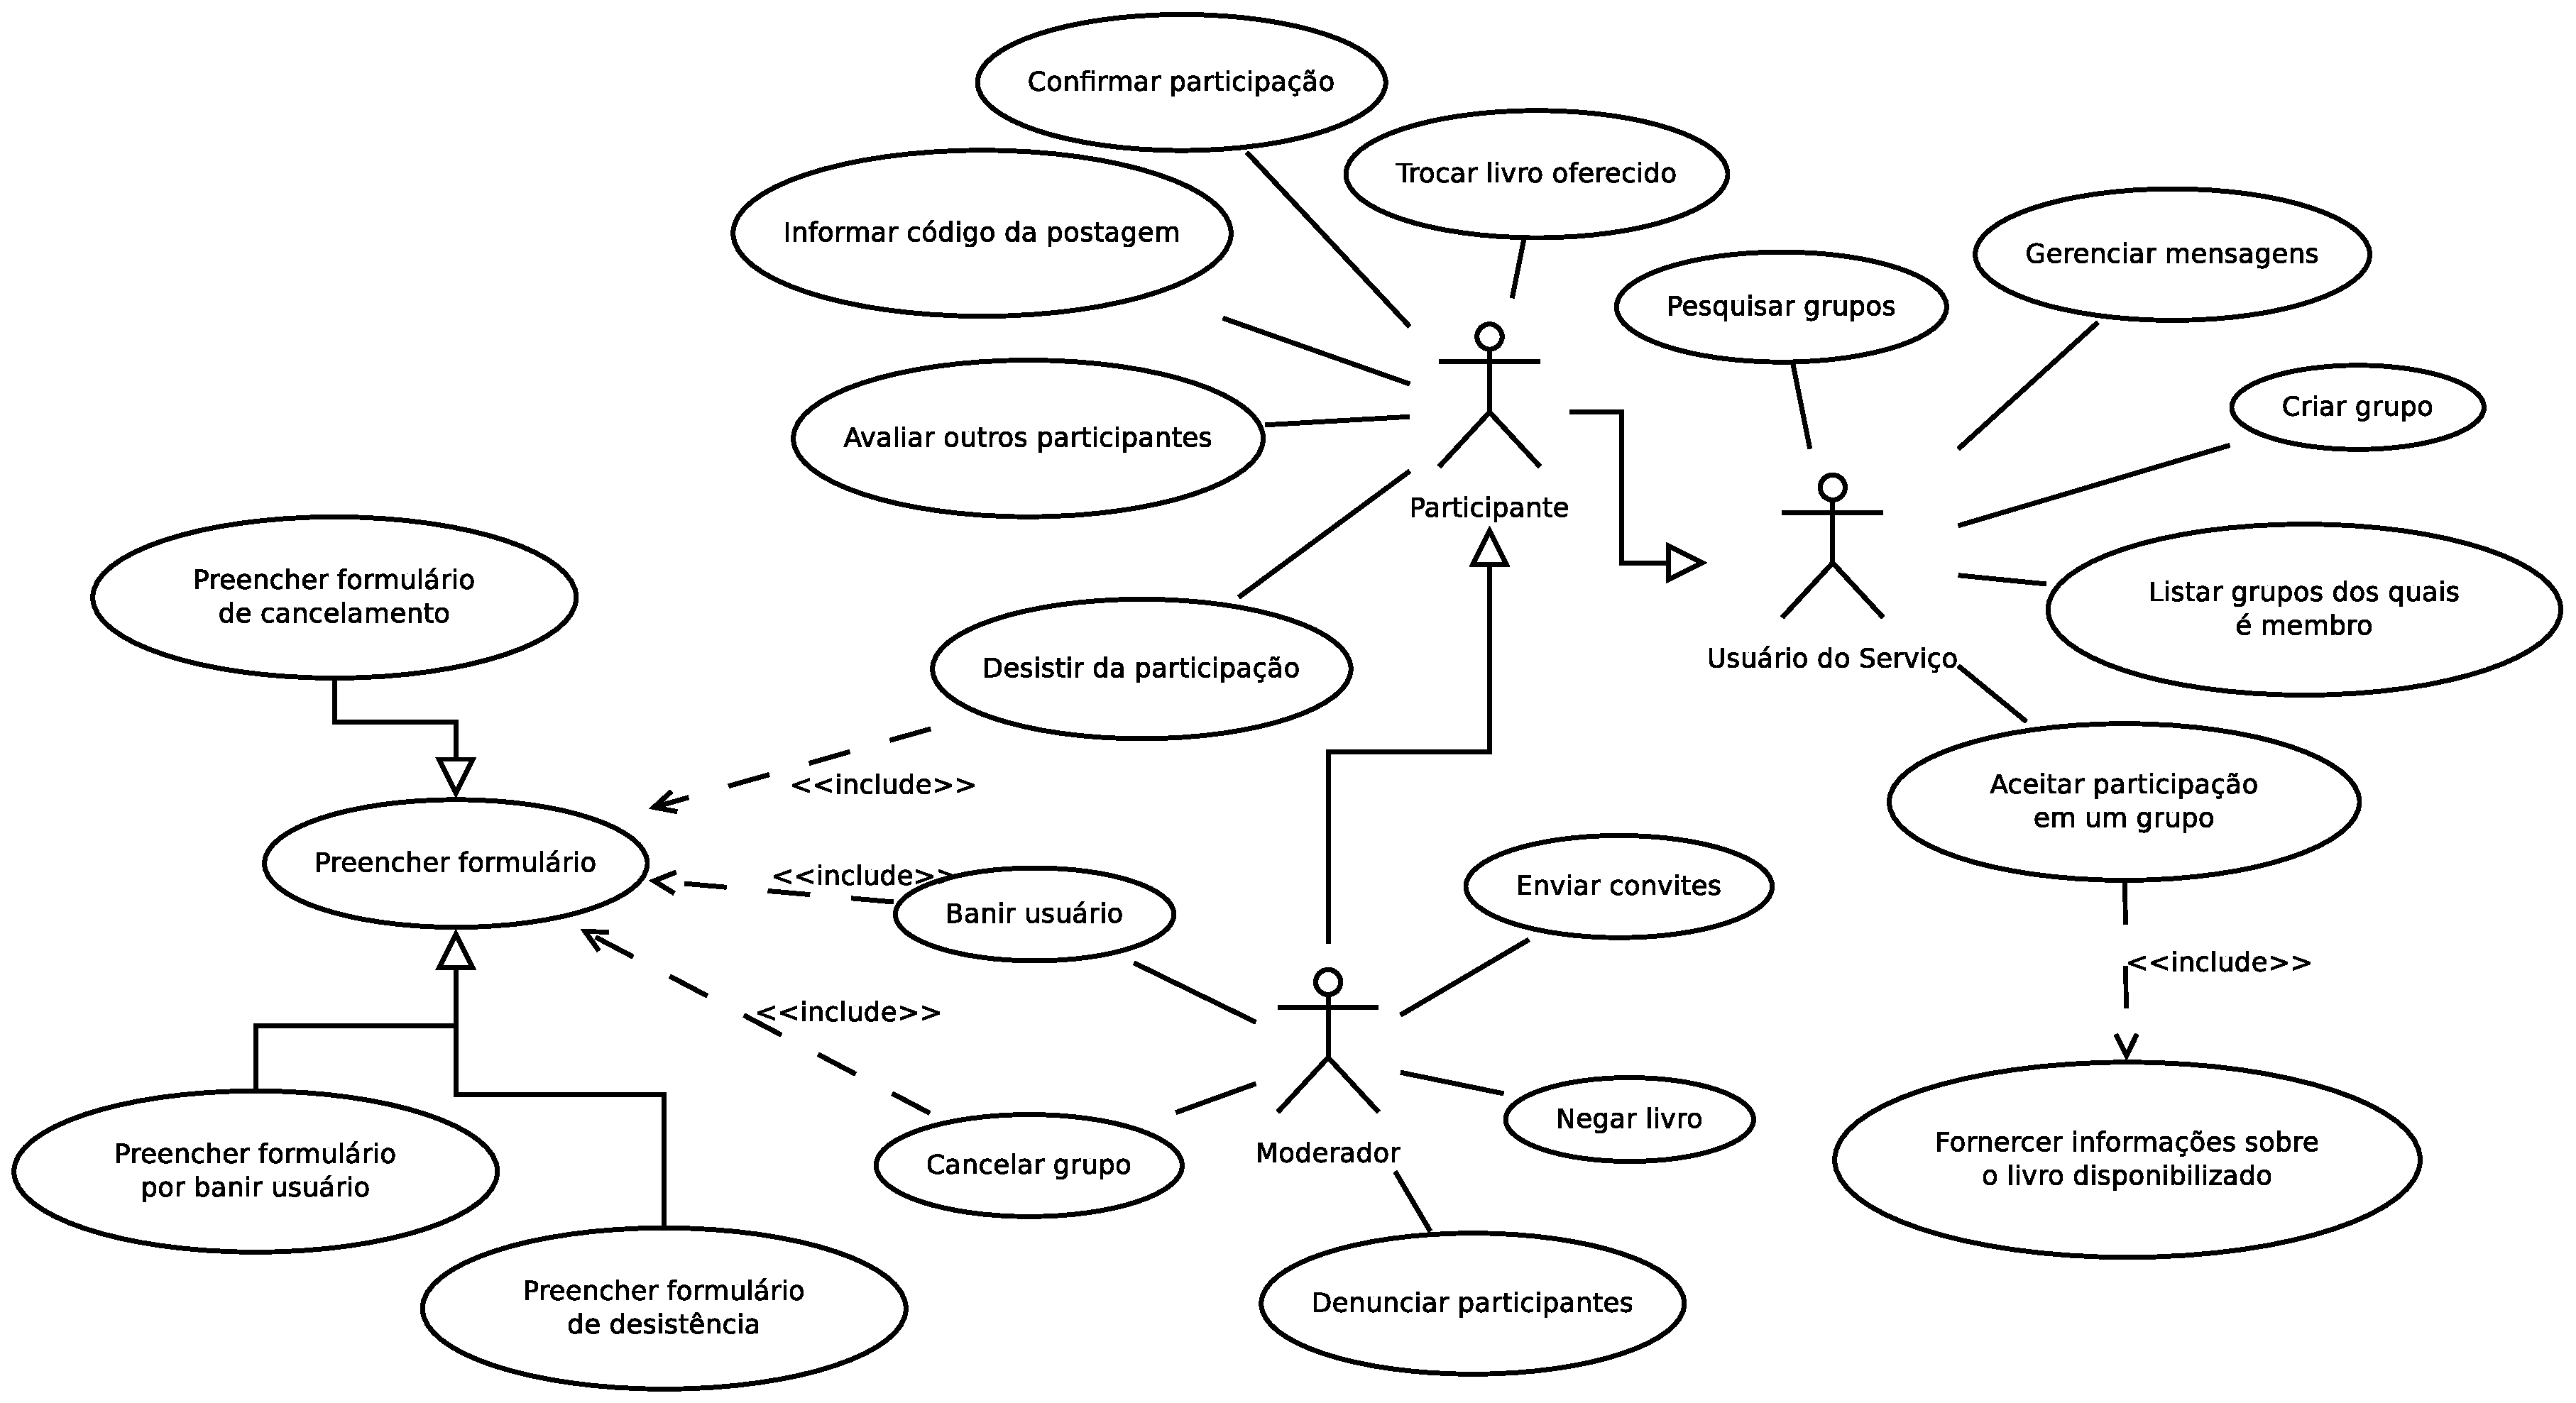
\includegraphics[angle=90,totalheight=\textheight]{casosDeUso.eps}
  \caption{Diagrama de Casos de Uso}
 \end{figure}
 
 \section{Classes}
 
 \begin{figure}[H]
  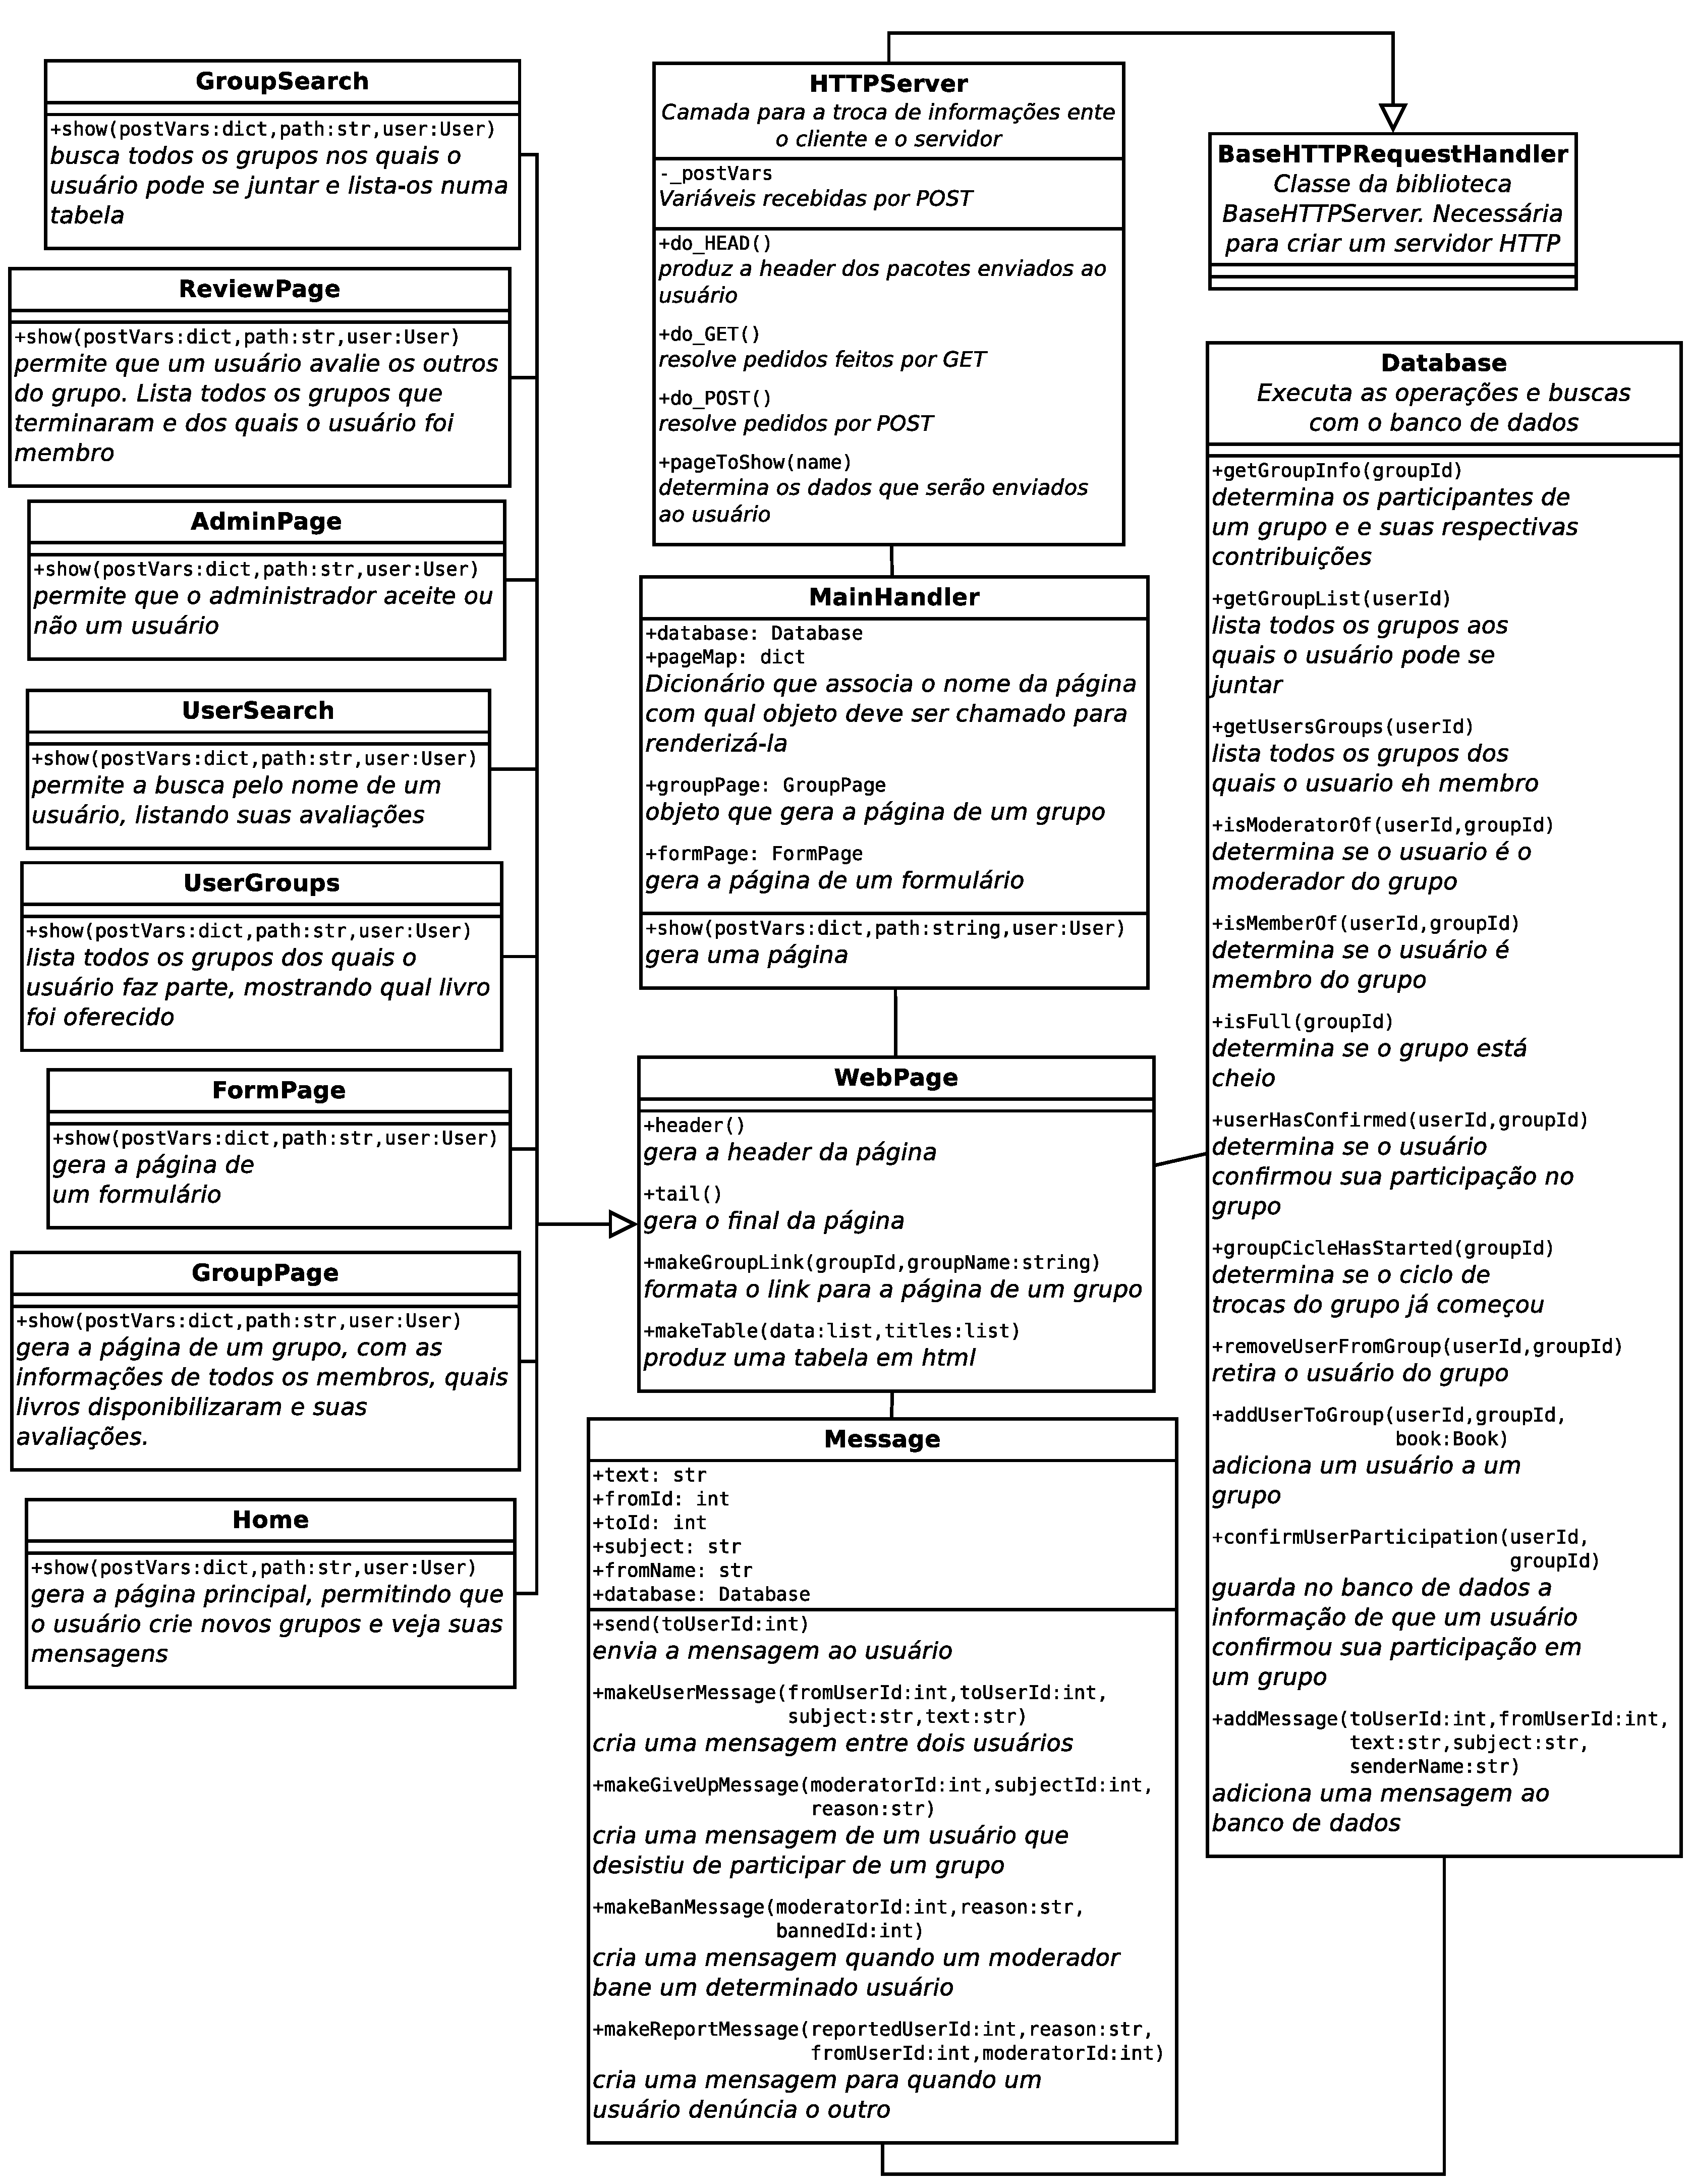
\includegraphics[totalheight=0.75\textheight]{classes.eps}
  \caption{Diagrama de Classes}
 \end{figure}
 
 \subsection{HTTPServer}
 
	\begin{description}
		\item [Super classe] BaseHTTPRequestHandler (parte da biblioteca BaseHTTPServer)
		\item [Propósito] Gerenciar os pedidos do usuário em baixo nível, isto é, recebe as informações de GET e POST e envia os dados necessários para que o usuário receba a informação pedida.
	\end{description}
	
	\subsubsection{Atributos}
		\begin{description}
		 \item [\_postVars] Armazena as variáveis passadas por POST
			\begin{description}
			 \item [Visibilidade] Privado
			\end{description}

		\end{description}

	
	\subsubsection{Métodos}
		\begin{description}
		 \item [do\_Head] produz a header dos pacotes enviados ao usuário
			\begin{description}
			 \item [visibilidade] Público
			 \item [retorno] NoneType
			\end{description}
			
			\item [do\_GET] resolve pedidos do tipo GET
			\begin{description}
			 \item [visibilidade] Público
			 \item [retorno] NoneType
			\end{description}
			
			\item [do\_POST] resolve pedidos do tipo POST. Atualiza postVars
			\begin{description}
			 \item [visibilidade] Público
			 \item [retorno] NoneType
			\end{description}
			
			\item [pageToShow] determina qual página foi pedida pelo usuário
			\begin{description}
			 \item [visibilidade] Privado
			 \item [entrada] \mbox{}
				\begin{description}
				 \item [name : str] Nome do conteúdo pedido
				\end{description}
				
			 \item [retorno : (str,str)] conteúdo da página e tipo do conteúdo
			\end{description}
		\end{description}
		
	\subsection{Database}
	
	\begin{description}
		\item [Propósito] Centralizar as pesquisas no banco de dados de forma que conhecimento deste seja apenas necessário dentro da classe.
	\end{description}
	
	\subsubsection{Atributos}
		\begin{description}
		 \item [host] Onde está o banco de dados
			\begin{description}
			 \item [Visibilidade] Público
			\end{description}
		
		\item [user] Nome de usuário para acessar o banco de dados
			\begin{description}
			 \item [Visibilidade] Público
			\end{description}
			
		\item [passwd] Senha para acessar o banco de dados
			\begin{description}
			 \item [Visibilidade] Público
			\end{description}
			
		\item [db] Nome da Database
			\begin{description}
			 \item [Visibilidade] Público
			\end{description}

		\end{description}

	
	\subsubsection{Métodos}
		\begin{description} % métodos
		 \item [getGroupInfo] determina as informações do grupo sobre os livros oferecidos, número de participantes e avaliações dos membros
			\begin{description} % propriedades
			 \item [visibilidade] Público
			 \item [Entrada] \mbox{}
				\begin{description} % entrada
				 \item [groupId : int] Id do grupo sobre o qual se quer os dados
				\end{description} % entrada
				
			 \item [retorno : T] onde T é uma Struct com os campos:
				\begin{description} % retorno
				 \item [books : (str,str) list] Título e autor de cada livro
				 \item [userInfo : (int,int) list] Avaliações positivas e negativas de cada usuário
				 \item [numMembers : int] Quantidade de membros do grupo
				\end{description} % retorno
				
			\end{description} % propriedades			
			
			\item [getGroupList] determina os grupos disponíveis ao usuário. Grupos disponíveis são aqueles que, além de não estarem cheios, são privados e o usuário recebeu um convite para eles ou então são públicos. 
			\begin{description}
			 \item [visibilidade] Público
			 \item [Entrada] \mbox{}
				\begin{description}
				 \item [userId : int] Id do usuário para o qual se está produzindo a lista de grupos disponíveis
				\end{description}
				
			 \item [retorno : T list] onde T é uma Struct com os campos:
			 \begin{description}
			  \item [id : int] Id do grupo
			  \item [name : str] Nome do grupo
			  \item [numMembers : int] Número de membros atualmente no grupo
			  \item [maxUsers : int] Número máximo de usuários que podem ser membros do grupo
			  \item [maxTime : int] Tempo máximo entre as trocas de livros (em dias)
			  \item [private : bool] Se o grupo é privado ou não
			 \end{description}

			\end{description}
			
			\item [getUsersGroups] lista todos os grupos dos quais o usuário faz parte
			\begin{description} % propriedades
			 \item [visibilidade] Público
			 \item [Entrada] \mbox{}
				\begin{description} % entrada
				 \item [userId : int] Id do usuário
				\end{description} % entrada
				
			 \item [retorno : T list ] onde T é uma Struct com os campos:
				\begin{description} % retorno
				 \item [book : str] Título do livro oferecido pelo usuário
				 \item [name : str] Nome do grupo
				 \item [id : int] Id do grupo
				\end{description} % retorno
				
			\end{description} % propriedades
			
			\item [getDestinationInfo] determina as informações do destinatário de uma troca 
			\begin{description} % propriedades
			 \item [visibilidade] Público
			 \item [Entrada] \mbox{}
				\begin{description} % entrada
				 \item [userId : int] Id do destinatário
				 \item [groupId : int] Id do grupo em que a troca ocorrerá
				\end{description} % entrada
				
			 \item [retorno : T ] onde T é uma Struct com os campos:
				\begin{description} % retorno
				 \item [address : str] Endereço para o qual o livro deve ser enviado
				 \item [date : str] Prazo limite para enviar o livro (formato: aaaa/mm/dd)
				\end{description} % retorno
				
			\end{description} % propriedades
			
			\item [isModeratorOf] determina se o usuário é o não moderador de um determinado grupo
			\begin{description} % propriedades
			 \item [visibilidade] Público
			 \item [Entrada] \mbox{}
				\begin{description} % entrada
				 \item [userId : int] Id do usuário
				 \item [groupId : int] Id do grupo
				\end{description} % entrada
				
			 \item [retorno : bool ] se o usuário é membro ou não do grupo
				
			\end{description} % propriedades
			
			\item [isMemberOf] determina se o usuário é membro do grupo
			\begin{description} % propriedades
			 \item [visibilidade] Público
			 \item [Entrada] \mbox{}
				\begin{description} % entrada
				 \item [userId : int] Id do usuário
				 \item [groupId : int] Id do grupo
				\end{description} % entrada
				
			 \item [retorno : bool ] se o usuário é membro ou não do grupo
				
			\end{description} % propriedades
			
			\item [isFull] determina se o grupo está cheio
			\begin{description} % propriedades
			 \item [visibilidade] Público
			 \item [Entrada] \mbox{}
				\begin{description} % entrada
				 \item [groupId : int] Id do grupo
				\end{description} % entrada
				
			 \item [retorno : bool ] se o grupo está cheio ou não
				
			\end{description} % propriedades
			
			\item [hasConfirmed] determina se o usuário já confirmou sua participação no grupo
			\begin{description} % propriedades
			 \item [visibilidade] Público
			 \item [Entrada] \mbox{}
				\begin{description} % entrada
				 \item [userId : int] Id do usuário
				 \item [groupId : int] Id do grupo
				\end{description} % entrada
				
			 \item [retorno : bool ] se o usuário confirmou ou não sua participação
				
			\end{description} % propriedades
			
			\item [groupCicleHasStarted] determina se o ciclo de trocas de um grupo iniciou
			\begin{description} % propriedades
			 \item [visibilidade] Público
			 \item [Entrada] \mbox{}
				\begin{description} % entrada
				 \item [ : int] Id do usuário
				 \item [ : int] Id do grupo
				\end{description} % entrada
				
			 \item [retorno : bool ] 
				
			\end{description} % propriedades
			
		\end{description} % métodos
 
\end{document}
